\documentclass{article}
\pagenumbering{gobble}
% \usepackage[bibstyle=phys,citestyle=numeric-comp,biblabel=brackets,sorting=none,backend=biber,bibencoding=auto]{biblatex}
% \addbibresource{references.bib}
% \DeclareFieldFormat{titlecase}{#1}%turn off sentence case

% \DeclareSourcemap{
%   \maps[datatype=bibtex, overwrite]{
%     \map{
%       \step[fieldset=extra, null]
%       \step[fieldset=note, null]
%     }
%   }
% }

% \usepackage{placeins}
% \usepackage{flafter}
% \usepackage[utf8]{inputenc}
\usepackage{mlmodern}
\usepackage[T1]{fontenc}

% \usepackage[english]{babel}
\usepackage{amsmath,amsfonts,amssymb}
\usepackage{mathrsfs}
\usepackage{clock}
\usepackage[clock]{ifsym}
% \usepackage{mathtools}
\usepackage{dcolumn}% Align table columns on decimal point
\usepackage{bm}
\usepackage[dvipsnames]{xcolor}
\usepackage{graphicx} % Allows for eps images
\usepackage{array}
\newcolumntype{C}[1]{>{\centering\let\newline\\\arraybackslash\hspace{0pt}}m{#1}}
\newcolumntype{L}[1]{>{\raggedright\let\newline\\\arraybackslash\hspace{0pt}}m{#1}}
\newcolumntype{M}[1]{>{\let\newline\\\arraybackslash\hspace{0pt}}m{#1}}
\usepackage{caption}
\usepackage{subcaption}
% \usepackage[caption=false,justification=justified]{subfig}
% \usepackage{authblk}
% \usepackage[framed, numbered]{matlab-prettifier}
\usepackage{float}
\usepackage{ragged2e}
% \usepackage{nidanfloat}
% \usepackage{stfloats}
% \usepackage{fixltx2e}
% \usepackage{url}
\usepackage{enumitem}
\usepackage{tensor}
\usepackage{centernot}
\usepackage{dsfont}
\usepackage[mathlines]{lineno}
% \linenumbers\relax % Commence numbering lines
% \usepackage[subfigure]{tocloft}
\usepackage{csquotes}
\usepackage{tikz}
\usetikzlibrary{shapes}
% \usetikzlibrary{quantikz}
\usetikzlibrary{arrows}
\usetikzlibrary{arrows.meta}
\usetikzlibrary{calc}
\usetikzlibrary{decorations.markings}
\usepackage{pgfplots}
\usepackage[outline]{contour}
\usepackage{tikz-feynman}
\usepackage{etoolbox}
% \usepackage{hyperref}
% \hypersetup{colorlinks=true,hyperfootnotes=false}
\pgfplotsset{compat=newest}
%\pgfplotsset{compat=1.17}
\usepackage[framemethod=tikz]{mdframed}
\definecolor{boxcolor}{HTML}{F5F5F5}

\renewenvironment{quote}%
  {\list{}{\leftmargin=-1.0em\rightmargin=-1.0em}\item[]}%
  {\endlist}

\def\QuantikzSeparationRow{0.8}

\usepackage{xparse}
\ExplSyntaxOn
\DeclareExpandableDocumentCommand{\IfNoValueOrEmptyTF}{mmm}
 {
  \IfNoValueTF{#1}{#2}
   {
    \tl_if_empty:nTF {#1} {#2} {#3}
   }
 }
\ExplSyntaxOff

\usepackage{xstring}
\def\replace#1#2#3{%
 \def\tmp##1#2{##1#3\tmp}%
   \tmp#1\stopreplace#2\stopreplace}
\def\stopreplace#1\stopreplace{}

\newcommand{\ChangeGreek}[1]{\begingroup
\let\theta\Theta
#1
\endgroup}

% Fix for spacing around \left and \right
% see: https://tex.stackexchange.com/questions/2607/spacing-around-left-and-right
\let\originalleft\left
\let\originalright\right
\renewcommand{\left}{\mathopen{}\mathclose\bgroup\originalleft}
\renewcommand{\right}{\aftergroup\egroup\originalright}

\definecolor{primarycolour}{HTML}{2266C0}
\definecolor{secondarycolour}{HTML}{B10061}
\definecolor{tertiarycolour}{HTML}{7000CC}
\definecolor{quaternarycolour}{HTML}{008A8A}
\newcommand{\ColA}{primarycolour}
\newcommand{\ColB}{secondarycolour}
\newcommand{\ColC}{tertiarycolour}
\newcommand{\ColD}{quaternarycolour}

% \input{macros.tex}

\DeclareDocumentCommand\Controlled{ m o o o }{
    \IfNoValueOrEmptyTF{#2}{}{\Control^{#2}}
    \IfNoValueOrEmptyTF{#3}{}{\Anticontrol^{#3}}
    \IfNoValueTF{#4}{#1}{{#1}^{#4}}
}
\tikzstyle{phantomhelper} = [
    rectangle,
    draw=none,
    fill=white,
    sloped,
    inner sep=0pt,
    outer sep=0pt,
    minimum width=3.75mm,
    minimum height=2.75mm,
]

\pgfplotscreateplotcyclelist{custom-list}{
    {cyan!0!magenta,mark=*},
    {cyan!33!magenta,mark=square*},
    {cyan!66!magenta,mark=triangle*},
    {cyan!100!magenta,mark=diamond*}%
}

%%% Wormhole mouths diagram:
\def\w{1}
\def\x{2}
\def\y{0.1}
\def\z{0.2}
\def\radius{1.625}
\def\sep{3}

% Style to set camera angle, like PGFPlots `view` style
\tikzset{viewport/.style 2 args={
    x={({cos(-#1)*\radius cm},{sin(-#1)*sin(#2)*\radius cm})},
    y={({-sin(-#1)*\radius cm},{cos(-#1)*sin(#2)*\radius cm})},
    z={(0,{cos(#2)*\radius cm})}
}}

% Convert from spherical to cartesian coordinates
\newcommand{\ToXYZ}[2]{
    {sin(#1)*cos(#2)}, % X coordinate
    {cos(#1)*cos(#2)}, % Y coordinate
    {sin(#2)}          % Z (vertical) coordinate
}

\def\rotation{20}
\def\offset{37.5}

%%% Penrose diagram:
% \usepackage{xparse} % Already included above as required for other purposes
\ExplSyntaxOn
\DeclareExpandableDocumentCommand{\eval}{m}{\fp_eval:n {#1}}
\ExplSyntaxOff

\tikzset{->-/.style={decoration={markings, mark=at position #1 with {\arrow{Latex[length=2.75mm,width=1.5mm]}}},postaction={decorate}}}

\def\sizing{10}%keep=10
\def\scaling{0.025}%fixed=0.025
\def\num{32}%25~101, test=5, good=32, okay=24
\def\spacing{0.035}%keep=0.0325~4, good=0.035
\def\domain{2.25}%min=1, max=10, fair=5, good=2.25
\def\granularity{129}%min=257, best=2049, test=17, good=129
\def\tension{0.5}
\def\bound{\eval{\scaling*(atand(\sizing*\domain)+atand(\sizing*\domain))}}
% Convert from Minkowski to Penrose-Carter coordinates
\newcommand{\ToUV}[2]{
    {\scaling*(atan(\sizing*(#1+#2))+atan(\sizing*(#1-#2)))},% T coordinate
    {\scaling*(atan(\sizing*(#1+#2))-atan(\sizing*(#1-#2)))} % X coordinate
}

%%% Bloch sphere:
\usepackage{blochsphere}
\usetikzlibrary{positioning,arrows,calc,math,angles,quotes}
\def\rotationSphere{-90}
\def\radiusSphere{2cm}
\def\psiLat{45}
\def\psiLon{45}

\input{./../../preamble/macros.tex}

\renewcommand{\large}{\normalsize}

% \usepackage{geometry}
% \geometry{
% paperwidth=8cm,
% paperheight=8cm,
% margin=0cm
% }

\begin{document}
\begin{figure}[b!]
\begin{center}
\begin{subfigure}[b]{0.45\textwidth}
\centering
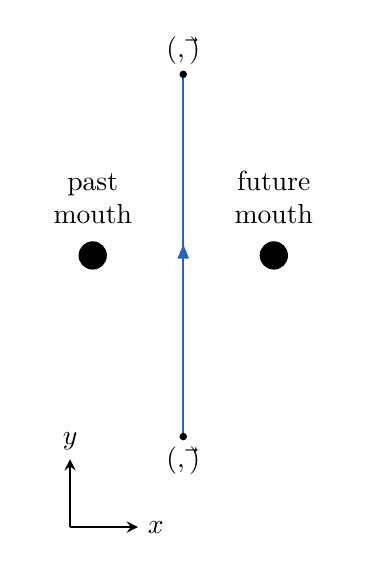
\begin{tikzpicture}[font=\fontsize{10}{12},scale=1.15]
    %\draw[step=1cm,gray,very thin] (-6,-6) grid (6,6);

    \node[isosceles triangle,shape border rotate = 90,isosceles triangle apex angle=45,scale=0.35,black,fill=\ColA] at (0,0) {};

    \draw[thick, \ColA] (0,-2) -- (0,2);

    \draw[black,fill=black] (0,-2) circle (0.035cm);
    \draw[black,fill=black] (0,2) circle (0.035cm);
    \draw[black,fill=black] (-1,0) circle (0.15cm);
    \draw[black,fill=black] (1,0) circle (0.15cm);

    \node[above] at (1,0.135) {\begin{tabular}{c} future \\ mouth \end{tabular}};
    \node[above] at (-1,0.135) {\begin{tabular}{c} past \\ mouth \end{tabular}};

    \node[below] at (0,-2) {$\left(\TimeInitial,\vec{\PositionInitial}\right)$};
    \node[above] at (0,2) {$\left(\TimeFinal,\vec{\PositionFinal}\right)$};
    %\node[above] at (0,-3.7) {$\mathrm{Evolution}\ \EvolutionA$};
    %\node[above] at (0,-4.25) {(a)};

    \node[right] at (-0.5,-3) {$x$};
    \node[above] at (-1.25,-2.25) {$y$};
    \draw [->,>=stealth,thick,black] (-1.25,-3) -- (-0.5,-3);
    \draw [->,>=stealth,thick,black] (-1.25,-3) -- (-1.25,-2.25);
\end{tikzpicture}
\caption{Evolution $\EvolutionNoninteracting$}
\end{subfigure}
\hspace*{0cm}
\begin{subfigure}[b]{0.45\textwidth}
\centering
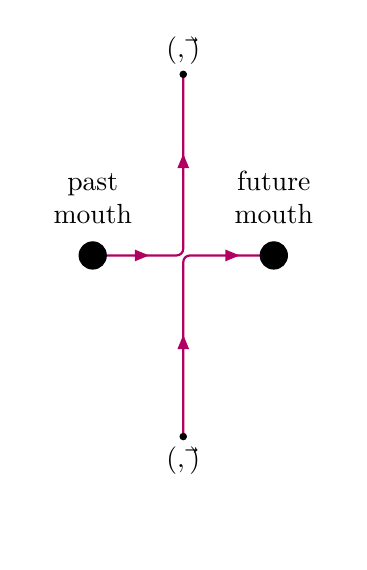
\begin{tikzpicture}[font=\fontsize{10}{12},scale=1.15]
    %\draw[step=1cm,gray,very thin] (-6,-6) grid (6,6);
    
    \node[isosceles triangle,shape border rotate = 90,isosceles triangle apex angle=45,scale=0.35,black,fill=\ColB] at (0,-1) {};
    \node[isosceles triangle,shape border rotate = 90,isosceles triangle apex angle=45,scale=0.35,black,fill=\ColB] at (0,1) {};
    \node[isosceles triangle,shape border rotate = 0,isosceles triangle apex angle=45,scale=0.35,black,fill=\ColB] at (0.5,0) {};
    \node[isosceles triangle,shape border rotate = 0,isosceles triangle apex angle=45,scale=0.35,black,fill=\ColB] at (-0.5,0) {};
    
    \draw[rounded corners=0.085cm, thick, \ColB] (-1,0) -- (0,0) -- (0,2);
    \draw[rounded corners=0.085cm, thick, \ColB] (0,-2) -- (0,0) -- (1,0);
    
    \draw[black,fill=black] (0,-2) circle (0.035cm);
    \draw[black,fill=black] (0,2) circle (0.035cm);
    \draw[black,fill=black] (-1,0) circle (0.15cm);
    \draw[black,fill=black] (1,0) circle (0.15cm);
    
    \node[above] at (1,0.135) {\begin{tabular}{c} future \\ mouth \end{tabular}};
    \node[above] at (-1,0.135) {\begin{tabular}{c} past \\ mouth \end{tabular}};
    
    \node[below] at (0,-2) {$\left(\TimeInitial,\vec{\PositionInitial}\right)$};
    \node[above] at (0,2) {$\left(\TimeFinal,\vec{\PositionFinal}\right)$};
    %\node[above] at (0,-3.7) {$\mathrm{Evolution}\ \EvolutionB$};
    %\node[above] at (0,-4.25) {(b)};
    
    \node[right,opacity=0] at (-0.5,-3) {$x$};
    \node[above,opacity=0] at (-1.25,-2.25) {$y$};
    \draw [->,>=stealth,thick,black,opacity=0] (-1.25,-3) -- (-0.5,-3);
    \draw [->,>=stealth,thick,black,opacity=0] (-1.25,-3) -- (-1.25,-2.25);
\end{tikzpicture}
\caption{Evolution $\EvolutionInteracting$}
\end{subfigure}
\end{center}
\end{figure}
\end{document}
